\chapter{Revisão Bibliográfica}
\label{cap:revisao}

\graphicspath{\currfiledir/figuras/} % caminho para as figuras deste capítulo

%=====================================================

Este capítulo apresenta uma revisão da literatura sobre bots, seu uso em contextos educacionais e as tecnologias relacionadas ao seu desenvolvimento, estabelecendo as bases conceituais para este trabalho.

O Capítulo está organizado da seguinte forma: a Seção \ref{sec:def-bots} apresenta a definição e componentes de bots, a Seção \ref{sec:class-bots} discute as classificações de bots, a Seção \ref{sec:bots-educ} aborda os bots no contexto educacional, incluindo os desafios do ensino remoto e aspectos de interação humano-computador na educação, a Seção \ref{sec:ferramentas} analisa bibliotecas e tecnologias para desenvolvimento de bots, a Seção \ref{sec:trab-rel} apresenta trabalhos relacionados, e finalmente, a Seção \ref{sec:objetivos} delineia os objetivos específicos deste trabalho com base nos conceitos apresentados.

%=====================================================

\section{Definição e Componentes de Bots}
\label{sec:def-bots}

Bots são programas automatizados projetados para interagir com usuários ou sistemas, realizando tarefas específicas com diferentes níveis de autonomia. Bots podem ser definidos como "aplicações que combinam uma interface conversacional com a capacidade de executar tarefas específicas para o usuário" \cite{dale2016}, ou também "uma aplicação que realiza certas tarefas repetitivas de maneira mais rápida que o ser humano" \cite{eslahi2012}.

A arquitetura de um bot pode ser descrita de diferentes maneiras na literatura, mas geralmente envolve um conjunto de componentes essenciais que trabalham juntos para processar a entrada do usuário, gerenciar o diaĺogo e gerar respostas apropriadas. Uma estrutura comum inclui como elementos principais (1) interface do usuário, (2) compreensão de linguagem natural, (3) gerenciador de diálogo, (4) integração com backend, e por fim (5) geração de linguagem natural \cite{huang2021}:

\begin{enumerate}
\item \textbf{Interface do Usuário (User Interface - UI)}: Este é o ponto de contato entre o usuário e o bot. A UI é responsável por receber a entrada do usuário (texto, voz, cliques em elementos gráficos) e apresentar as respostas do bot de forma compreensível. Pode variar desde simples janelas de chat baseadas em texto até interfaces de voz sofisticadas ou GUIs interativas.
\item \textbf{Compreensão de Linguagem Natural (Natural Language Understanding - NLU)}: Este componente é crucial para interpretar a entrada do usuário em linguagem natural. Ele analisa o texto ou a fala para identificar a intenção do usuário (o que o usuário quer fazer) e extrair informações relevantes, conhecidas como entidades (por exemplo, datas, locais, nomes). O NLU transforma a entrada não estruturada do usuário em dados estruturados que o bot pode processar.
\item \textbf{Gerenciador de Diálogo (Dialogue Manager - DM)}: O DM mantém o estado do diálogo (o contexto da conversa), rastreia o histórico de interações e decide qual ação tomar a seguir com base na intenção identificada pelo NLU e nas regras de negócio ou na lógica conversacional definida. Isso pode envolver fazer perguntas de esclarecimento, acessar a base de conhecimento, chamar uma API externa ou gerar uma resposta. O DM pode ser implementado usando abordagens baseadas em regras ou modelos de aprendizado de máquina mais complexos.
\item \textbf{Integração com Backend e Base de Conhecimento (Backend Integration \& Knowledge Base)}: Para realizar tarefas úteis e fornecer informações precisas, os chatbots frequentemente precisam interagir com sistemas externos e acessar dados. A integração com o backend permite que o bot se conecte a APIs, bancos de dados, sistemas de CRM, ou outras fontes de informação e serviços. Essa base de conhecimento pode incluir conhecimento estático (pré-programado), conhecimento dinâmico (acessado em tempo real via APIs), conhecimento contextual (histórico do usuário) e até conhecimento colaborativo (gerado pelo usuário). É importante a integração com o backend para acessar essas informações e executar ações.
\item \textbf{Geração de Resposta (Response Generation - RG)}: Uma vez que o Gerenciador de Diálogo decide a resposta a ser dada, o componente RG a transforma em linguagem natural (texto ou fala) para ser apresentada ao usuário através da Interface do Usuário. A complexidade do RG pode variar desde o uso de modelos de resposta pré-definidos até a geração dinâmica de sentenças complexas.
\end{enumerate}

\begin{figure}[!htb]
\centering
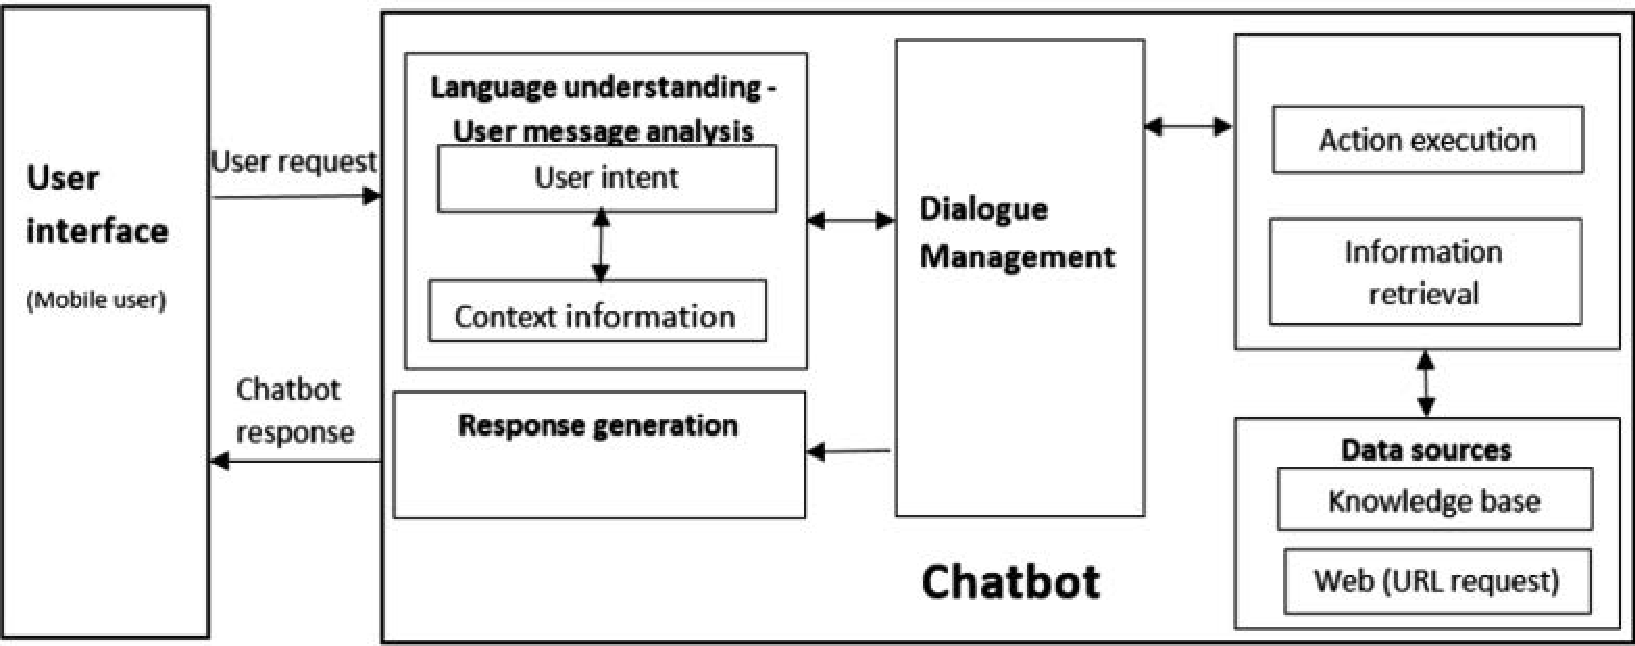
\includegraphics[width=12cm]{huang-arquitetura.pdf}
\caption{Arquitetura de um chatbot por Huang et al. \cite{huang2021}.}
\label{fig:bot-arch}
\end{figure}


%=====================================================

\section{Classificações de Bots}
\label{sec:class-bots}

Existem diversas formas de classificar bots, dependendo de suas características, funcionalidades e aplicações. Os bots podem ser classificados de acordo com seu propósito principal \cite{lebeuf2019}, ou de acordo com a sua funcionalidade primária \cite{seering2018}.

\begin{table}[H]
\centering
\label{tab:classificacao_bots}
\begin{tabular}{|p{4.2cm}|p{9cm}|}
\hline
\textbf{Propósito}\cite{lebeuf2019}& \textbf{Descrição} \\
\hline
Bots generalistas & Executam uma ampla variedade de tarefas, como responder perguntas gerais e executar comandos simples. \\
\hline
Bots transacionais & Realizam transações com sistemas externos, como bots bancários ou de compras. \\
\hline
Bots informacionais & Fornecem informações e respondem perguntas específicas dos usuários. \\
\hline
Bots de produtividade & Automatizam tarefas repetitivas, como lembretes ou agendamentos. \\
\hline
Bots de colaboração & Facilitam a interação e colaboração entre usuários, geralmente em ambientes de comunicação. \\
\hline
\textbf{Funcionalidade}\cite{seering2018} & \textbf{Descrição} \\
\hline
Tarefas administrativas & Auxiliam na organização de atividades, como agendar reuniões e gerenciar compromissos. \\
\hline
Entretenimento & Proporcionam atividades lúdicas, como jogos ou interações divertidas. \\
\hline
Funcionalidade e qualidade & Aumentam a eficiência de serviços, como bots de suporte técnico ou de coleta de feedback. \\
\hline
Comunidade & Moderam e gerenciam interações em comunidades online. \\
\hline
Arquivadores & Organizam e recuperam informações, como documentos e registros de mensagens. \\
\hline
\end{tabular}
\caption{Classificação de bots segundo propósito e funcionalidade}
\end{table}

\noindent Este trabalho concentra-se em bots do tipo "produtividade" e "colaboração" como propósito, e "funcionalidade e qualidade" como funcionalidade. O foco é a sua aplicação dentro do contexto educacional, onde eles podem atuar como assistentes virtuais que facilitam a interação entre alunos e professores, a fim de promover um ambiente remoto de aprendizagem mais dinâmico e interativo.

%=====================================================

\section{Bots no Contexto Educacional}
\label{sec:bots-educ}

Na educação, os bots têm sido utilizados para diversos propósitos, desde fornecer suporte administrativo até oferecer experiências de aprendizado personalizadas. Os bots educacionais podem transformar a experiência de aprendizagem ao oferecer suporte contínuo e personalizado que seria impraticável para um professor humano fornecer a todos os alunos simultaneamente \cite{zawacki2019}.

Estudos recentes têm explorado aplicações educacionais específicas de bots. Por exemplo, o uso de chatbots para melhorar a retenção de conhecimento em estudantes universitários \cite{okonkwo2021}, e aumentar o engajamento em cursos online abertos e massivos (MOOCs) \cite{han2022}.

De uma maneira geral, bots educacionais são particularmente eficazes quando (1) fornecem feedback imediato aos alunos, (2) oferecem disponibilidade contínua para assistência, (3) personalizam a experiência de aprendizado, (4) reduzem a carga cognitiva dos instrutores e (5) permitem que os instrutores se concentrem em atividades pedagógicas e interativas \cite{silva2024}.

A seguir, exploramos quatro dimensões importantes relacionadas ao uso de bots educacionais: os desafios específicos do ensino remoto que podem ser mitigados por essas ferramentas, os princípios de interação humano-computador relevantes para o design de bots educacionais eficazes, os princípios fundamentais para a interação mediada por bots na educação, e o papel dos dashboards como ferramentas de controle pedagógico.

%-----------------------------------------------------

\subsection{Desafios do Ensino Remoto}
\label{subsec:desafios}

O ensino remoto apresenta desafios únicos que podem ser parcialmente mitigados pelo uso de tecnologias interativas como bots. Aqui se faz distinção entre "ensino remoto emergencial" e educação online planejada, destacando que muitas instituições foram forçadas a adotar o primeiro modelo durante a pandemia de COVID-19, sem tempo adequado para planejamento \cite{hodges2020}\cite{fabiane2024}.

\noindent Entre os principais desafios identificados estão \cite{fabiane2024}:

\begin{itemize}
\item Limitações tecnológicas e acesso desigual
\item Competências digitais insuficientes de professores e alunos
\item Falta de estrutura para avaliação eficaz
\item Dificuldade em manter o engajamento dos alunos
\item Ausência de interação social e senso de comunidade
\end{itemize}

\noindent Tecnologias como bots podem preencher algumas dessas lacunas ao proporcionar uma interface natural e contínua entre os participantes do processo educacional, oferecendo um canal adicional de comunicação e suporte tanto para alunos quanto para professores \cite{winkler2018}.

%-----------------------------------------------------

\subsection{Interação Humano-Computador na Educação}
\label{subsec:ihc}

Estudos em IHC destacam a importância de sistemas que se ajustem ao comportamento e às necessidades dos usuários \cite{roy1987}. Na educação, isso implica em promover interfaces que permitam participação ativa, acessibilidade e adaptabilidade aos estilos de aprendizagem dos alunos.

Norman \cite{norman2013} enfatiza o conceito de design centrado no usuário, onde a tecnologia deve se adaptar às necessidades humanas e não o contrário. Aplicado ao contexto educacional, este princípio sugere que os bots devem ser projetados considerando as necessidades pedagógicas específicas e as limitações cognitivas dos alunos.

Bots educacionais se encaixam nesse contexto por serem acessíveis e flexíveis na forma de interação. Interfaces conversacionais podem reduzir a carga cognitiva associada à navegação em sistemas educacionais complexos, permitindo que os alunos se concentrem no conteúdo do aprendizado em vez de na interface \cite{sweller2011}.

%-----------------------------------------------------

\subsection{Princípios para Interação Mediada por Bots na Educação}
\label{subsec:principios}

Com base na literatura sobre bots educacionais e metodologias ativas, surgem três princípios fundamentais emergem como pilares para o design de interações eficazes mediadas por bots em ambientes educacionais:

\begin{enumerate}
\item \textbf{Comunicação multidirecional}: Um bot educacional eficaz não deve apenas transmitir informações do professor para os alunos, mas também facilitar o retorno dos alunos para o professor, criando um ciclo contínuo de feedback. Esse princípio alinha-se com a concepção de aprendizagem dialógica \cite{calvo2013}, onde o conhecimento é construído através da interação bidirecional entre educador e educando.
\item \textbf{Engajamento ativo}: Através de mecânicas interativas, o bot deve estimular constantemente a participação dos alunos, transformando-os de receptores passivos a agentes ativos no processo de aprendizagem. Este princípio está fundamentado nas teorias construtivistas de aprendizagem \cite{piaget1970}, que enfatizam a importância da experiência prática e da participação na construção do conhecimento.
\item \textbf{Adaptação contextual}: O sistema deve se ajustar ao ritmo da aula e às necessidades específicas da disciplina, oferecendo diferentes modos de interação conforme o momento pedagógico. Tecnologias educacionais eficazes devem ser flexíveis o suficiente para se adaptarem a diferentes contextos pedagógicos e estilos de aprendizagem \cite{winkler2018}.
\end{enumerate}

Estes princípios fornecem uma base teórica para o design de bots educacionais que efetivamente aprimoram o processo de aprendizagem, especialmente em contextos de metodologias ativas onde a participação e o engajamento dos alunos são essenciais.

%-----------------------------------------------------

\subsection{Dashboards como Ferramenta de Controle Pedagógico}
\label{subsec:dashboards}

Um elemento crucial no design de bots educacionais é a interface de controle que permite aos educadores gerenciar o fluxo das interações. Os dashboards pedagógicos surgem como uma solução para esta necessidade, oferecendo uma visão consolidada das atividades e permitindo intervenções em tempo real sem interromper o fluxo da aula \cite{verbert2013}.

Dashboards de aprendizagem são "displays únicos que agregam diferentes indicadores sobre aprendiz, atividades de aprendizagem e/ou contexto de aprendizagem em uma ou múltiplas visualizações" \cite{verbert2013}. No contexto de bots educacionais, estes dashboards evoluem para se tornarem não apenas ferramentas de visualização, mas interfaces de comando que permitem aos professores:

\begin{enumerate}
\item \textbf{Orquestrar atividades}: Iniciar e controlar sequências de aprendizagem sem necessidade de inserir comandos em chats públicos
\item \textbf{Monitorar em tempo real}: Visualizar métricas de engajamento e compreensão durante a aula
\item \textbf{Receber alertas}: Ser notificado sobre padrões que exijam intervenção pedagógica
\item \textbf{Personalizar interações}: Adaptar atividades com base nas necessidades observadas
\item \textbf{Analisar resultados}: Obter relatórios detalhados após as sessões
\end{enumerate}

\begin{figure}[H]
\centering
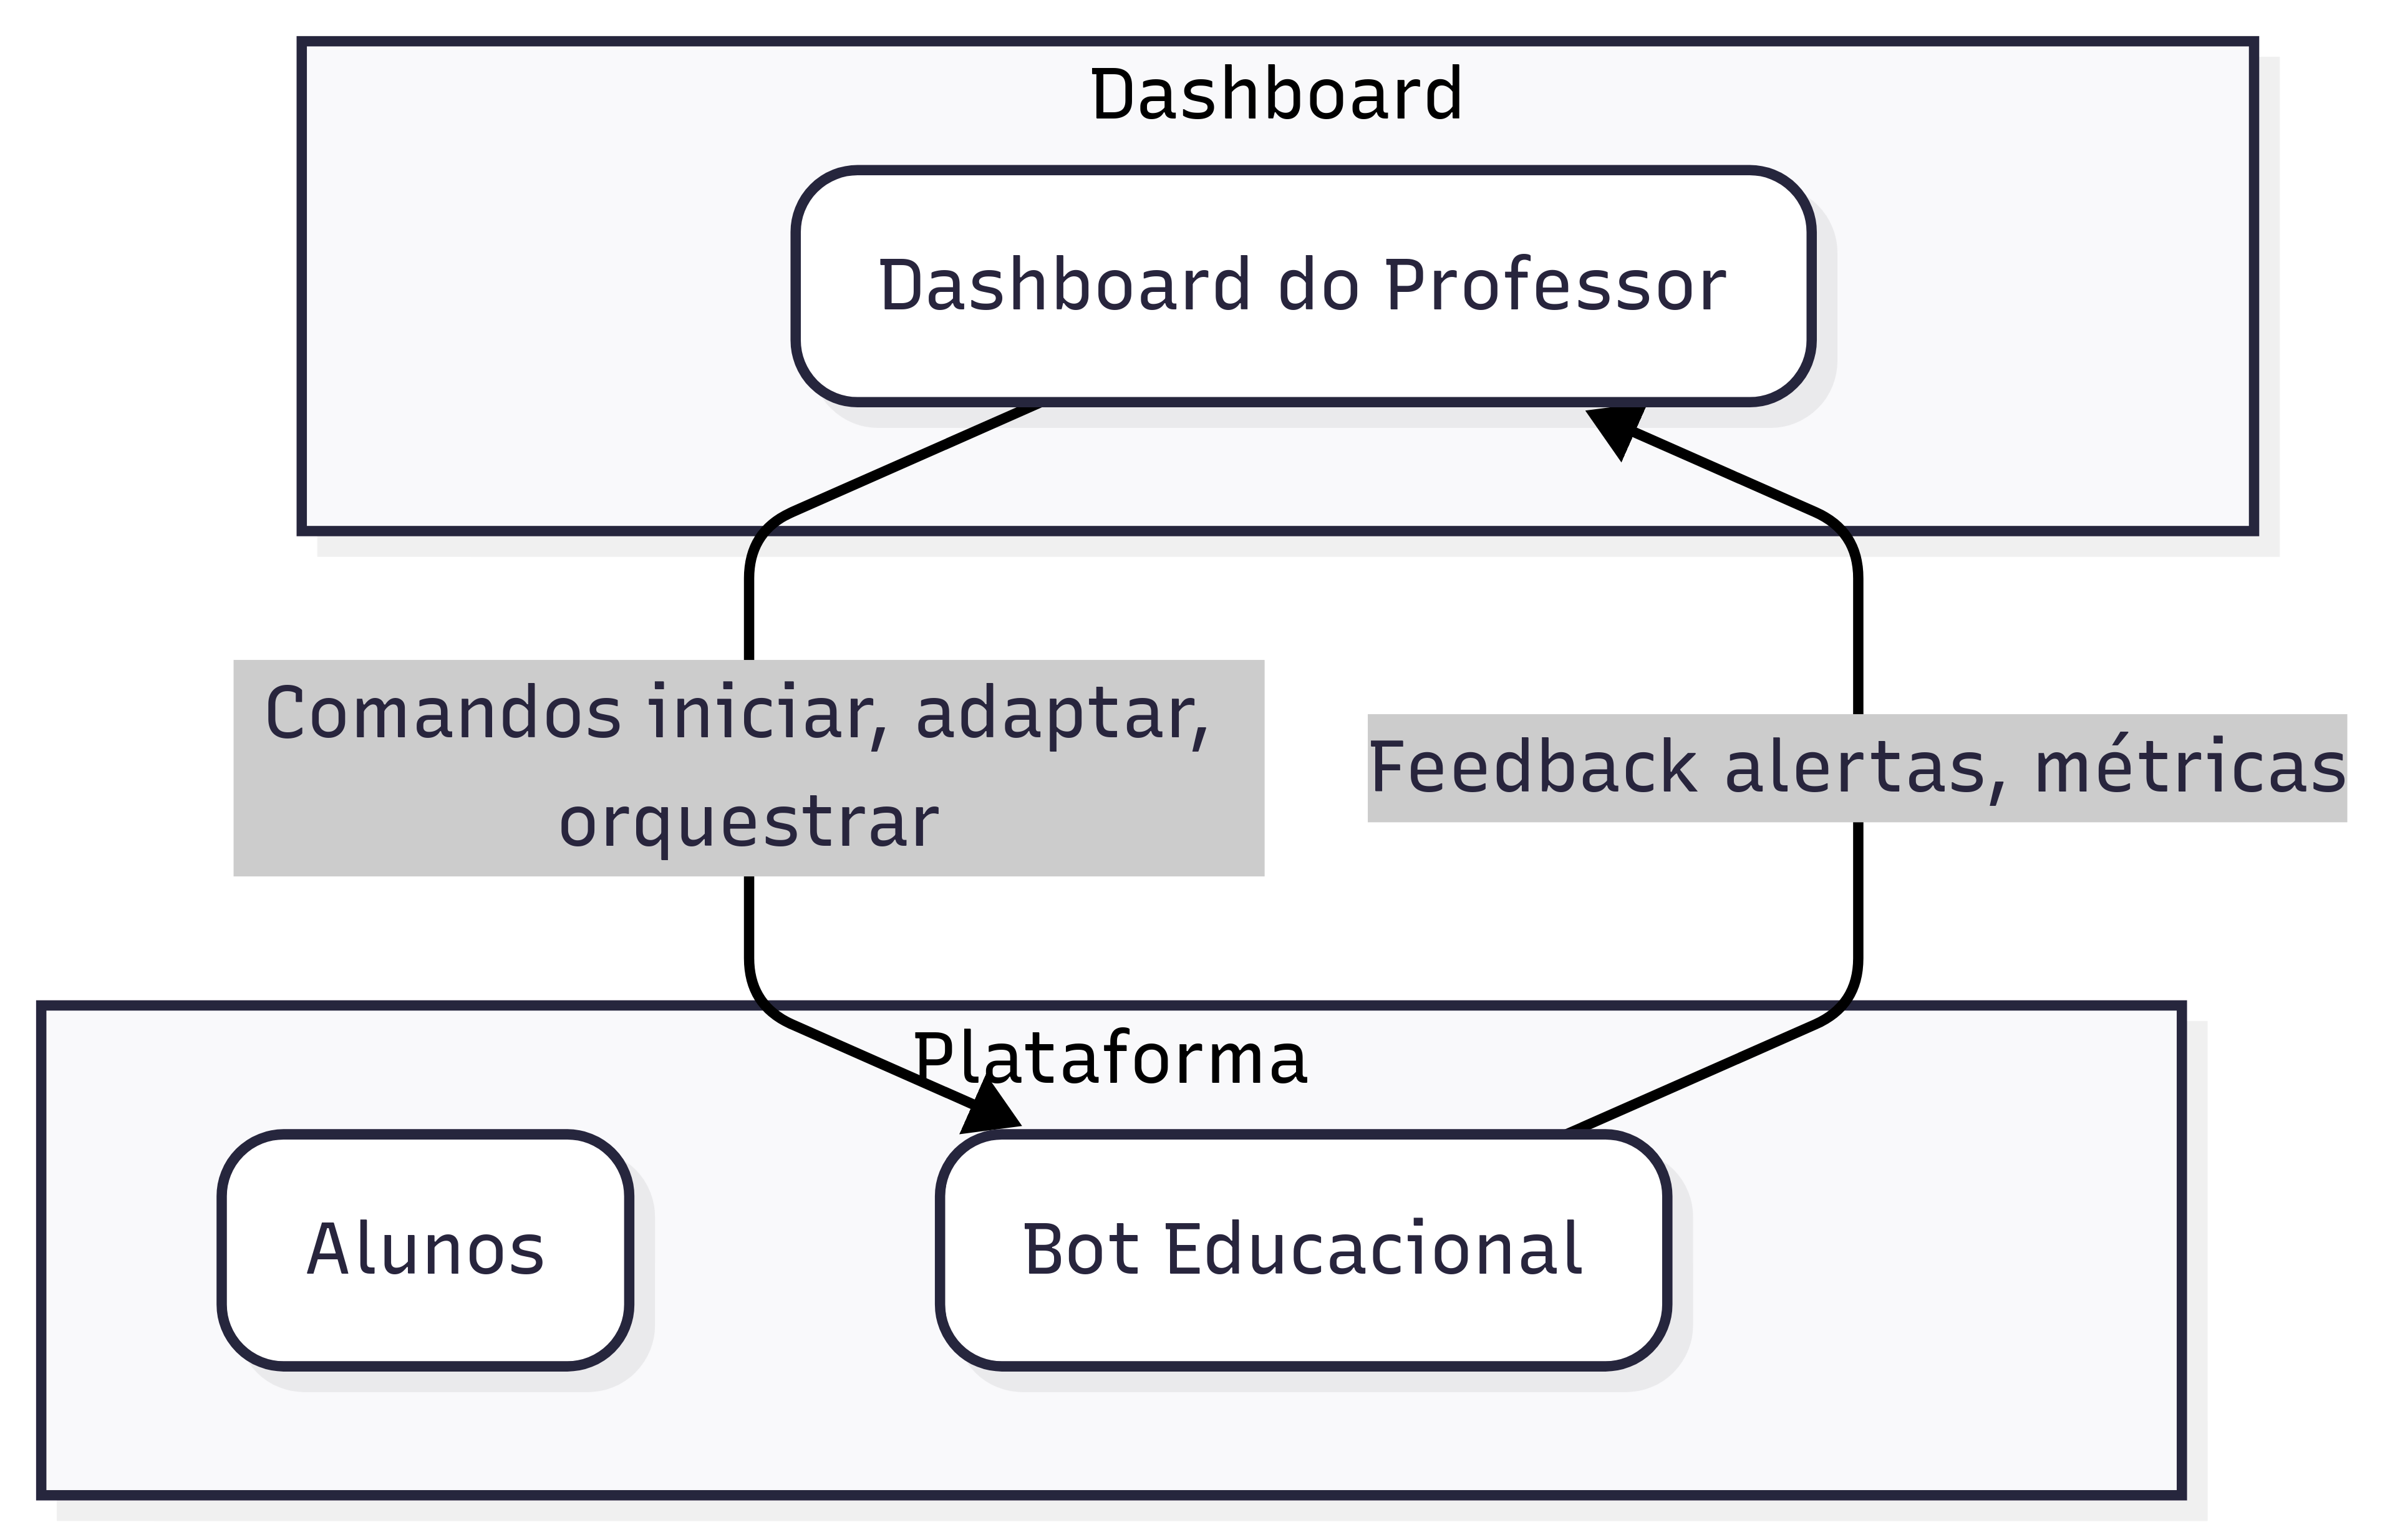
\includegraphics[width=12cm]{relacao-dashboard-bot.png}
\caption{Relação entre o bot educacional e o dashboard de controle pedagógico.}
\label{fig:dashboard-bot}
\end{figure}

Esta abordagem separa claramente o canal de comando (dashboard, visível apenas para o professor) do canal de interação (plataforma de comunicação, visível para todos os participantes), seguindo o princípio de "separação de interesses" como essencial para ambientes de aprendizagem tecnologicamente mediados. A eficácia desse modelo de interação será avaliada em experimentos controlados, onde participantes assumirão papéis de professor e alunos, interagindo em um ambiente de sala de aula simulado.

%=====================================================

\section{Ferramentas para Desenvolvimento de Bots no Discord}
\label{sec:ferramentas}

Existem várias ferramentas para desenvolver bots, dentre elas destacamos bibliotecas específicas para a plataforma do Discord, cada uma com suas particularidades e casos de uso apropriados, (1) JavaScript/Node.js, (2) Python e (3) C. 

\begin{enumerate}
\item \textbf{Discord.js}\cite{discordjs}: Uma biblioteca JavaScript/Node.js que oferece abstração de alto nível para interação com a API do Discord. É rica em recursos e possui uma comunidade ativa, sendo adequada para desenvolvedores que preferem desenvolvimento rápido.
\item \textbf{Discord.py}\cite{discordpy}: Equivalente ao Discord.js, mas para a linguagem Python. Oferece abstrações semelhantes e é amplamente utilizada para desenvolvimento de bots no Discord.
\item \textbf{Concord}\cite{muller}: Uma biblioteca em C que fornece acesso de baixo nível à API do Discord, desenvolvida pelo autor deste trabalho. Diferentemente das opções anteriores, a Concord prioriza desempenho e controle direto sobre a API, sendo apropriada para aplicações que demandam eficiência computacional e controle granular.
\end{enumerate}

No contexto deste estudo, foi escolhida a biblioteca Concord, por sua implementação na linguagem C, que oferece um equilíbrio entre abstração e controle que a torna adequada para uma ampla gama de aplicações \cite{kernighan1988}. No contexto educacional, C é frequentemente utilizada como linguagem de ensino em cursos de programação devido à sua sintaxe fundamental que expõe conceitos importantes de ciência da computação, como gerenciamento de memória e estruturas de dados básicas \cite{kernighan1988}.

Para estudos futuros, é importante considerar o uso de linguagens de mais alto nível como Python, JavaScript ou Go, que podem oferecer desenvolvimento mais rápido e maior facilidade de manutenção, especialmente em projetos onde a curva de aprendizado reduzida seja prioritária em relação ao desempenho bruto. A linguagem de programação em contextos educacionais deve equilibrar considerações pedagógicas, praticidade de implementação e objetivos específicos do projeto \cite{pears2007}.

%=====================================================

\section{Trabalhos Relacionados}
\label{sec:trab-rel}

Diversos pesquisadores têm explorado o uso de bots em contextos educacionais:

Hien et al. \cite{hien2018} desenvolveram um bot para suporte a alunos em um curso de programação, que respondia a dúvidas sobre conceitos e sintaxe. Os resultados mostraram uma redução no tempo de resposta para dúvidas comuns e um aumento na satisfação dos alunos com o suporte recebido.

Demetriadis et al. \cite{demetriadis2018} implementaram um agente conversacional para auxiliar alunos em atividades colaborativas de resolução de problemas. O estudo demonstrou que grupos apoiados pelo bot apresentaram maior engajamento e melhores resultados de aprendizagem em comparação com grupos sem suporte automatizado.

Yin et al. \cite{yin2024} compararam o fornecimento de feedback formativo aos alunos por chatbot e professor. A avaliação indicou que alunos que receberam feedback regularmente do chatbot apresentaram maior interesse de aprendizagem, além de redução da carga cognitiva necessária para aprender conceitos complexos.

Um trabalho particularmente relevante é o de Winkler e Söllner \cite{winkler2018}, que propõe diretrizes para o design de chatbots educacionais focados em metodologias ativas, destacando a importância de promover interações que estimulem o pensamento crítico e a reflexão.

%=====================================================

\section{Objetivos do Trabalho}
\label{sec:objetivos}

Com base na revisão bibliográfica apresentada, este trabalho tem como objetivo desenvolver e avaliar um bot educacional assistivo e conversacional para plataformas de colaboração, especificamente o Discord, que facilite a implementação de metodologias ativas em ambientes de ensino remoto.

Os objetivos específicos incluem:

\begin{enumerate}
\item \textbf{Desenvolver um bot educacional} que incorpore os três princípios fundamentais para interação mediada discutidos na Seção \ref{subsec:principios}: comunicação multidirecional, engajamento ativo e adaptação contextual.
\item \textbf{Implementar funcionalidades específicas} que abordem diretamente os desafios do ensino remoto identificados na Seção \ref{subsec:desafios}, com foco especial em manter o engajamento dos alunos, facilitar o feedback imediato e promover interações sociais significativas em ambientes virtuais.
\item \textbf{Proporcionar uma integração não-invasiva} da ferramenta ao fluxo de trabalho docente, aplicando os princípios de design centrado no usuário e minimizando a carga cognitiva adicional, conforme destacado nos estudos de IHC educacional na Seção \ref{subsec:ihc}.
\item \textbf{Criar uma prova de conceito funcional} utilizando tecnologias adequadas ao contexto educacional, considerando aspectos de eficiência, portabilidade e manutenção, conforme discutido na Seção \ref{sec:ferramentas}.
\item \textbf{Estabelecer uma metodologia de avaliação experimental} com participantes reais assumindo os papéis de professor e alunos, onde o professor utiliza o dashboard de controle enquanto os alunos interagem com o bot em um ambiente de sala de aula simulado, permitindo mensurar a eficácia da solução em situações próximas ao uso real, combinando métricas quantitativas e qualitativas, inspirada nos trabalhos apresentados na Seção \ref{sec:trab-rel}.
\end{enumerate}

Tecnicamente, o desenvolvimento será realizado utilizando a biblioteca Concord em C (desenvolvida pelo autor), aproveitando suas vantagens em termos de controle granular sobre a API do Discord e sua relevância educacional, conforme discutido na Seção \ref{sec:ferramentas}.

Este trabalho se diferencia dos esforços anteriores apresentados na Seção \ref{sec:trab-rel} por seu foco específico em facilitar metodologias ativas em ambientes remotos, com ênfase na integração não-invasiva à prática docente e sua metodologia de avaliação que simula condições reais de uso. Enquanto outros trabalhos têm explorado bots para responder dúvidas ou fornecer feedback automatizado, esta proposta busca transformar a própria dinâmica de interação durante as aulas síncronas, com uma avaliação sistemática em um ambiente controlado.

Os próximos capítulos detalham a concepção e implementação do bot (\ref{cap:bot}), bem como sua avaliação através da metodologia experimental com participantes em diferentes papéis (Capítulo 4), demonstrando como os conceitos teóricos discutidos neste capítulo se manifestam na prática educacional.